%! TeX program = lualatex
\documentclass[12pt, landscape]{scrartcl}

\usepackage[paperheight=12in,paperwidth=18in,margin=0in,heightrounded,showframe]{geometry}
\usepackage{graphicx}
\usepackage[osf]{libertine}
\usepackage{lettrine}
\usepackage[dvipsnames]{xcolor} 
\usepackage[object=vectorian]{pgfornament}
\usepackage{pgfornament-han}
% \usepackage[document]{ragged2e}
\usepackage{background}
\usepackage{pifont}
\usepackage{soul}

\usetikzlibrary{calc}
\definecolor{fondpaille}{cmyk}{0,0,0.1,0}
\definecolor{calpolypomonagreen}{rgb}{0.12, 0.3, 0.17}
\definecolor{forestgreen(traditional)}{rgb}{0.0, 0.27, 0.13}
\definecolor{darkgreen}{rgb}{0.0, 0.2, 0.13}

%%%%%%%%%%%%%%%%%%%%%%%%
%%% First background %%%
%%%%%%%%%%%%%%%%%%%%%%%%
% \backgroundsetup{
% scale=1,
% opacity=1,
% angle=0,
% color=darkgreen,
% contents={%
% \begin{tikzpicture}[every node/.style={inner sep=0pt}]
% \node[anchor=north west](CNW)
% at (current page.north west) {\pgfornament[width=4.5cm]{63}};
% \node[anchor=north east](CNE)
% at (current page.north east) {\pgfornament[width=4.5cm,symmetry=v]{63}};
% \node[anchor=south west](CSW)
% at (current page.south west) {\pgfornament[width=4.5cm,symmetry=h]{63}};
% \node[anchor=south east](CSE)
% at (current page.south east) {\pgfornament[width=4.5cm,symmetry=c]{63}};
% %
% % \node[anchor=north, rotate=0](CNW)  at (current page.north)
% % {\pgfornament[width=10cm,symmetry=c]{71}}; 
% % \node[anchor=south, rotate=0](CNW)  at (current page.south)
% % {\pgfornament[width=10cm,symmetry=c]{71}}; 
% %
% \node[shift={(5.0cm,0cm)},anchor=north west, rotate=0](CNW)  at (current page.north west)
% {\pgfornament[width=10cm,symmetry=c]{71}}; 
% \node[shift={(5.0cm,0cm)},anchor=south west, rotate=0](CNW)  at (current page.south west)
% {\pgfornament[width=10cm,symmetry=c]{71}}; 
% %
% \node[shift={(-5.0cm,0cm)},anchor=north east, rotate=0](CNW)  at (current page.north east)
% {\pgfornament[width=10cm,symmetry=c]{71}}; 
% \node[shift={(-5.0cm,0cm)},anchor=south east, rotate=0](CNW)  at (current page.south east)
% {\pgfornament[width=10cm,symmetry=c]{71}}; 
% %
% \node[shift={(13.5cm,0cm)},anchor=north west, rotate=0](CNW)  at (current page.north west)
% {\pgfornament[width=10cm,symmetry=c]{71}}; 
% \node[shift={(13.5cm,0cm)},anchor=south west, rotate=0](CNW)  at (current page.south west)
% {\pgfornament[width=10cm,symmetry=c]{71}}; 
% %
% \node[shift={(-13.5cm,0cm)},anchor=north east, rotate=0](CNW)  at (current page.north east)
% {\pgfornament[width=10cm,symmetry=c]{71}}; 
% \node[shift={(-13.5cm,0cm)},anchor=south east, rotate=0](CNW)  at (current page.south east)
% {\pgfornament[width=10cm,symmetry=c]{71}}; 
% %
% \node[shift={(0cm,5.2cm)}, anchor= south east, rotate=270](CSE) at (current page.south west)
% {\pgfornament[width=10cm,symmetry=c]{71}}; 
% \node[shift={(0cm,-5.2cm)}, anchor= south west, rotate=270](CNE) at (current page.north west)
% {\pgfornament[width=10cm,symmetry=c]{71}}; 
% %
% \node[shift={(0cm,5.2cm)}, anchor= south west, rotate=90](CSE) at (current page.south east)
% {\pgfornament[width=10cm,symmetry=c]{71}}; 
% \node[shift={(0cm,-5.2cm)}, anchor= south east, rotate=90](CNE) at (current page.north east)
% {\pgfornament[width=10cm,symmetry=c]{71}};
%     % 
% \end{tikzpicture}%
%   }
% }

% %%%%%%%%%%%%%%%%%%%%%%%%%%
% %%% Second background  %%%
% %%%%%%%%%%%%%%%%%%%%%%%%%%
% \backgroundsetup{
% scale=1,
% opacity=1,
% angle=0,
% color=darkgreen,
% contents={%
% \begin{tikzpicture}[every node/.style={inner sep=0pt}]
%     \pgfmathsetmacro{\cornersize}{6cm}
%     \pgfmathsetmacro{\edgesize}{1.5cm}
%     \pgfmathsetmacro{\widthstart}{-floor((\textwidth - 2*\cornersize)/\edgesize/2)*(\edgesize/1cm)}
%     \pgfmathsetmacro{\widthstep}{\widthstart + 2*(\edgesize/1cm)}
%     \pgfmathsetmacro{\widthend}{-\widthstart - 2*(\edgesize/1cm)}
%     \pgfmathsetmacro{\heightstart}{-floor((\textheight - 2*\cornersize)/\edgesize/2)*(\edgesize/1cm)}
%     \pgfmathsetmacro{\heightstep}{\heightstart + 2*(\edgesize/1cm)}
%     \pgfmathsetmacro{\heightend}{-\heightstart - 2*(\edgesize/1cm)}
%     \pgfmathsetmacro{\step}{(\edgesize/1cm)}
%     \pgfmathsetmacro{\offx}{0.4}
%     \pgfmathsetmacro{\offy}{0.5}
%     \def\picsize{2.3cm}
%     % Corners ornaments
%     \node[anchor=north west](CNW)
%     at (current page.north west) {\pgfornament[width=\cornersize]{63}};
%     \node[anchor=north east](CNE)
%     at (current page.north east) {\pgfornament[width=\cornersize,symmetry=v]{63}};
%     \node[anchor=south west](CSW)
%     at (current page.south west) {\pgfornament[width=\cornersize,symmetry=h]{63}};
%     \node[anchor=south east](CSE)
%     at (current page.south east) {\pgfornament[width=\cornersize,symmetry=c]{63}};
%     Top
%     \foreach \x in {\widthstart,\widthstep,...,\widthend}
%     {\node[shift={(\x,0cm)},anchor=north west](CNW)  at (current page.north)
%     {\pgfornament[width=\edgesize,symmetry=v]{19}}; 
%     \node[shift={(\x+\step,0cm)},anchor=north west](CNW)  at (current page.north)
%     {\pgfornament[width=\edgesize,symmetry=h]{19}}; 
%     % Bottom
%     \node[shift={(\x,0cm)},anchor=south west](CNW)  at (current page.south)
%     {\pgfornament[width=\edgesize,symmetry=v]{19}};
%     \node[shift={(\x+\step,0cm)},anchor=south west](CNW)  at (current page.south)
%     {\pgfornament[width=\edgesize,symmetry=h]{19}}; }
%     % Left
%     \foreach \x in {\heightstart,\heightstep,...,\heightend}
%     {\node[shift={(0cm,\x)},anchor=south west](CSW)  at (current page.west)
%     {\pgfornament[width=\edgesize,symmetry=v]{19}}; 
%     \node[shift={(0cm,\x+\step)},anchor=south west](CSW)  at (current page.west)
%     {\pgfornament[width=\edgesize,symmetry=h]{19}}; 
%     % Right
%     \node[shift={(0cm,\x)},anchor=south east](CNW)  at (current page.east)
%     {\pgfornament[width=\edgesize,symmetry=v]{19}};
%     \node[shift={(0cm,\x+\step)},anchor=south east](CNW)  at (current page.east)
%     {\pgfornament[width=\edgesize,symmetry=h]{19}}; }
%     % 
%     % \node at (6,6) {\Huge \bfseries \heightend};
% \end{tikzpicture}
%   }
% }

%%%%%%%%%%%%%%%%%%%%%%%%%%
%%% Third background  %%%
%%%%%%%%%%%%%%%%%%%%%%%%%%
\backgroundsetup{
scale=1,
opacity=1,
angle=0,
color=darkgreen,
contents={%
\begin{tikzpicture}[every node/.style={inner sep=0pt}]
    \pgfmathsetmacro{\cornersize}{6cm}
    \pgfmathsetmacro{\edgesize}{6cm}
    \pgfmathsetmacro{\widthstart}{-((\textwidth - 2*\cornersize)/\edgesize/2)*(\edgesize/1cm)}
    % \pgfmathsetmacro{\widthstep}{\widthstart + 0.924*(\edgesize/1cm)}
    \pgfmathsetmacro{\widthstep}{\widthstart + (-2*\widthstart - (\edgesize/1cm))/(ceil(-2*\widthstart/(\edgesize/1cm))}
    \pgfmathsetmacro{\widthend}{-\widthstart - (\edgesize/1cm)}
    \pgfmathsetmacro{\heightstart}{-((\textheight - 2*\cornersize)/\edgesize/2)*(\edgesize/1cm)}
    \pgfmathsetmacro{\heightstep}{\heightstart + (-2*\heightstart - (\edgesize/1cm))/(ceil(-2*\heightstart/(\edgesize/1cm))}
    \pgfmathsetmacro{\heightend}{-\heightstart - (\edgesize/1cm)}
    \pgfmathsetmacro{\step}{(\edgesize/1cm)}
    \pgfmathsetmacro{\offx}{0.4}
    \pgfmathsetmacro{\offy}{0.5}
    \pgfmathsetmacro{\lineoff}{1.2}
    \def\picsize{2.3cm}
    % Corners ornaments
    \node[anchor=north west](CNW)
    at (current page.north west) {\pgfornamenthan[width=\cornersize]{28}};
    \node[anchor=north east](CNE)
    at (current page.north east) {\pgfornamenthan[width=\cornersize,symmetry=v]{28}};
    \node[anchor=south west](CSW)
    at (current page.south west) {\pgfornamenthan[width=\cornersize,symmetry=h]{28}};
    \node[anchor=south east](CSE)
    at (current page.south east) {\pgfornamenthan[width=\cornersize,symmetry=c]{28}};
    % Corners pictures
    \node[shift={(\offx,-\offy)}, anchor=north west](CNW)
    at (current page.north west) {
\includegraphics[width=\picsize]{../Figures/image1.png}};
    \node[shift={(-\offx,-\offy)}, anchor=north east](CNE)
    at (current page.north east) {
\includegraphics[width=\picsize]{../Figures/image2.png}};
    \node[shift={(\offx,\offy)}, anchor=south west](CSW)
    at (current page.south west) {
\includegraphics[width=\picsize]{../Figures/image3.png}};
    \node[shift={(-\offx,\offy)}, anchor=south east](CSE)
    at (current page.south east) {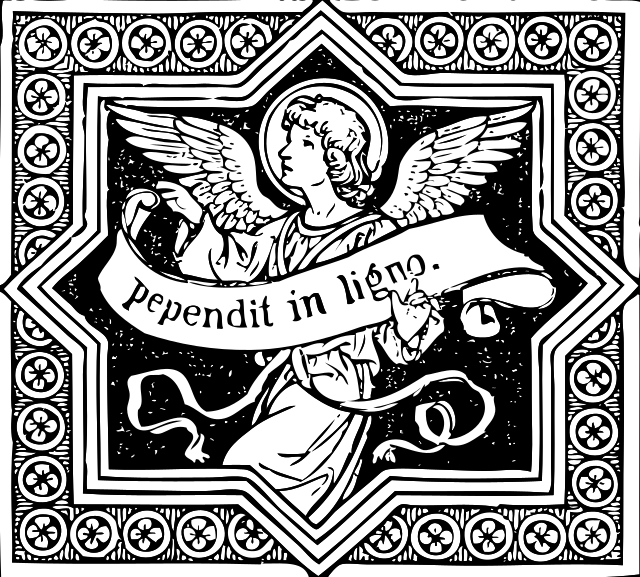
\includegraphics[width=\picsize]{../Figures/image4.png}};
    % Top
    \foreach \x in {\widthstart,\widthstep,...,\widthend}
    {\node[shift={(\x,-\lineoff)},anchor=north west](CNW)  at (current page.north)
    {\pgfornamenthan[width=\edgesize,symmetry=v]{30}}; 
    % Bottom
    \node[shift={(\x,\lineoff)},anchor=south west](CNW)  at (current page.south)
    {\pgfornamenthan[width=\edgesize,symmetry=v]{30}};}
    % Left
    \foreach \x in {\heightstart,\heightstep,...,\heightend}
    {\node[shift={(\lineoff,\x)},anchor=north west, rotate=90](CSW)  at (current page.west)
    {\pgfornamenthan[width=\edgesize,symmetry=v]{30}}; 
    % Right
    \node[shift={(-\lineoff,\x)},anchor=north east, rotate=270](CNW)  at (current page.east)
    {\pgfornamenthan[width=\edgesize,symmetry=v]{30}}; }
    % 
    % \node[anchor=south,shift={(0,0)}] at (current page.south)
    %     (se) {\pgfornamenthan[scale=0.4,symmetry=c]{30}};
    % \node at (6,6) {\Huge \bfseries \heightend};
\end{tikzpicture}
  }
}

\tolerance=1
\emergencystretch=\maxdimen
\hyphenpenalty=10000
\hbadness=10000

\setulcolor{Maroon}
\setlength{\parindent}{0pt}

\newcommand{\cross}{\textcolor{red}{\raisebox{-1mm}{\scalebox{1.5}{\ding{64}}}}}
\newcommand{\amen}{\textcolor{Maroon}{Amen.}}
\newcommand{\initial}[2]{\lettrine[lines=3]{\color{Maroon}#1}{\bfseries\color{Maroon}#2}}
\newcommand{\gap}{\vspace{0.3cm}}
\newcommand{\bend}[1]{\ul{#1}}

%%%%%%%%%%%%%%%%%%%%%%%%%%%%%%%%%%%%%%%%%%%%%%%%%%%%%%%%%%%%%%%%%%%%%%%%%%%%%%%%

\begin{document}

\thispagestyle{empty}

\pagecolor{fondpaille}
% \color{Maroon}
\color{darkgreen}
\large

\begin{center}

	\begin{minipage}[t]{0.29\linewidth}

		\vspace*{2.2cm}

		\initial{\hspace*{2cm}G}{loria} in~excelsis \bend{Deo}. Et~in~terra pax
		hominibus bonae voluntatis. Laudamus te. Benedicimus te. \bend{Adoramus
			te}. Glorificamus te. \bend{Gratias agimus tibi} propter magnam gloriam
		tuam. Domine Deus, Rex caelestis, Deus Pater omnipotens. Domine Fili
		unigenite, \bend{Jesu Christe}. Domine Deus, Agnus Dei, Filius Patris.
		Qui tollis peccata mundi, miserere nobis. Qui tollis peccata mundi,
		\bend{suscipe deprecationem nostram}. Qui sedes ad~dexteram Patris,
		miserere nobis. Quoniam tu solus Sanctus. Tu solus Dominus. Tu solus
		Altissimus, \bend{Jesu Christe}. Cum Sancto \cross~ Spiritu in~gloria
		Dei Patris. \amen

		\gap

		\initial{M}{unda} cor meum, ac~labia mea, omnipotens Deus, qui labia
		Isaiae Prophetae calculo mundasti ignito: ita me~tua grata miseratione
		dignare mundare, ut~sanctum Evangelium tuum digne valeam nuntiare. Per
		Christum Dominum nostrum. \amen

		\gap

		\initial{I}{ube}, Domine benedicere. Dominus sit in~corde meo et~in~
		labiis meis: ut~digne et~competenter annuntiem Evangelium suum. \amen

		\gap

		\initial{C}{redo} in~unum \bend{Deum}, Patrem omnipotentem, factorem
		caeli et~terrae, visibilium omnium, et~invisibilium. Et~in~unum Dominum
		\bend{Jesum Christum}, Filium Dei unigenitum. Et~ex Patre natum ante
		omnia saecula. Deum de~Deo, lumen de~lumine, Deum verum de~Deo vero.
		Genitum, non factum, consubstantialem Patri: per quem omnia facta sunt.
		Qui propter nos homines, et~propter nostram salutem descendit de~caelis.
		\textcolor{Maroon}{\bfseries\scshape Et~incarnatus est de~spiritu sancto
			ex~maria virgine: et~homo factus est.} Crucifixus etiam pro nobis, sub
		Pontio Pilato passus, et~sepultus est. Et~resurrexit tertia die,
		secundum Scripturas. Et~ascendit in~caelum: sedet ad~dexteram Patris.
		Et~iterum venturus est cum gloria, judicare vivos, et~mortuos: cujus
		regni non erit finis. Et~in~Spiritum Sanctum, Dominum et~vivificantem:
		qui ex~Patre Filioque procedit. Qui cum Patre et~Filio \bend{simul
			adoratur} et~conglorificatur: qui locutus est per Prophetas. Et~unam,
		sanctam, catholicam et~apostolicam Ecclesiam. Confiteor unum baptisma
		in~remissionem
		% 
		\hspace*{2cm} \parbox{0.85\linewidth}{ \smallskip peccatorum.
			Et~exspecto resurrectionem mortuorum. Et~vitam \cross~venturi saeculi.
			\amen}

		% \vspace*{0.25em}
		% \hfill
		% \begin{minipage}{0.85\linewidth}
		% 	peccatorum. Et~exspecto resurrectionem mortuorum. Et~vitam \cross~venturi
		% 	saeculi.
		% 	\amen
		% \end{minipage}


	\end{minipage}
	\hspace*{0.8cm}
	\begin{minipage}[t]{0.25\linewidth}
		%
		\vspace*{2.2cm}
		%
		\begin{center}
			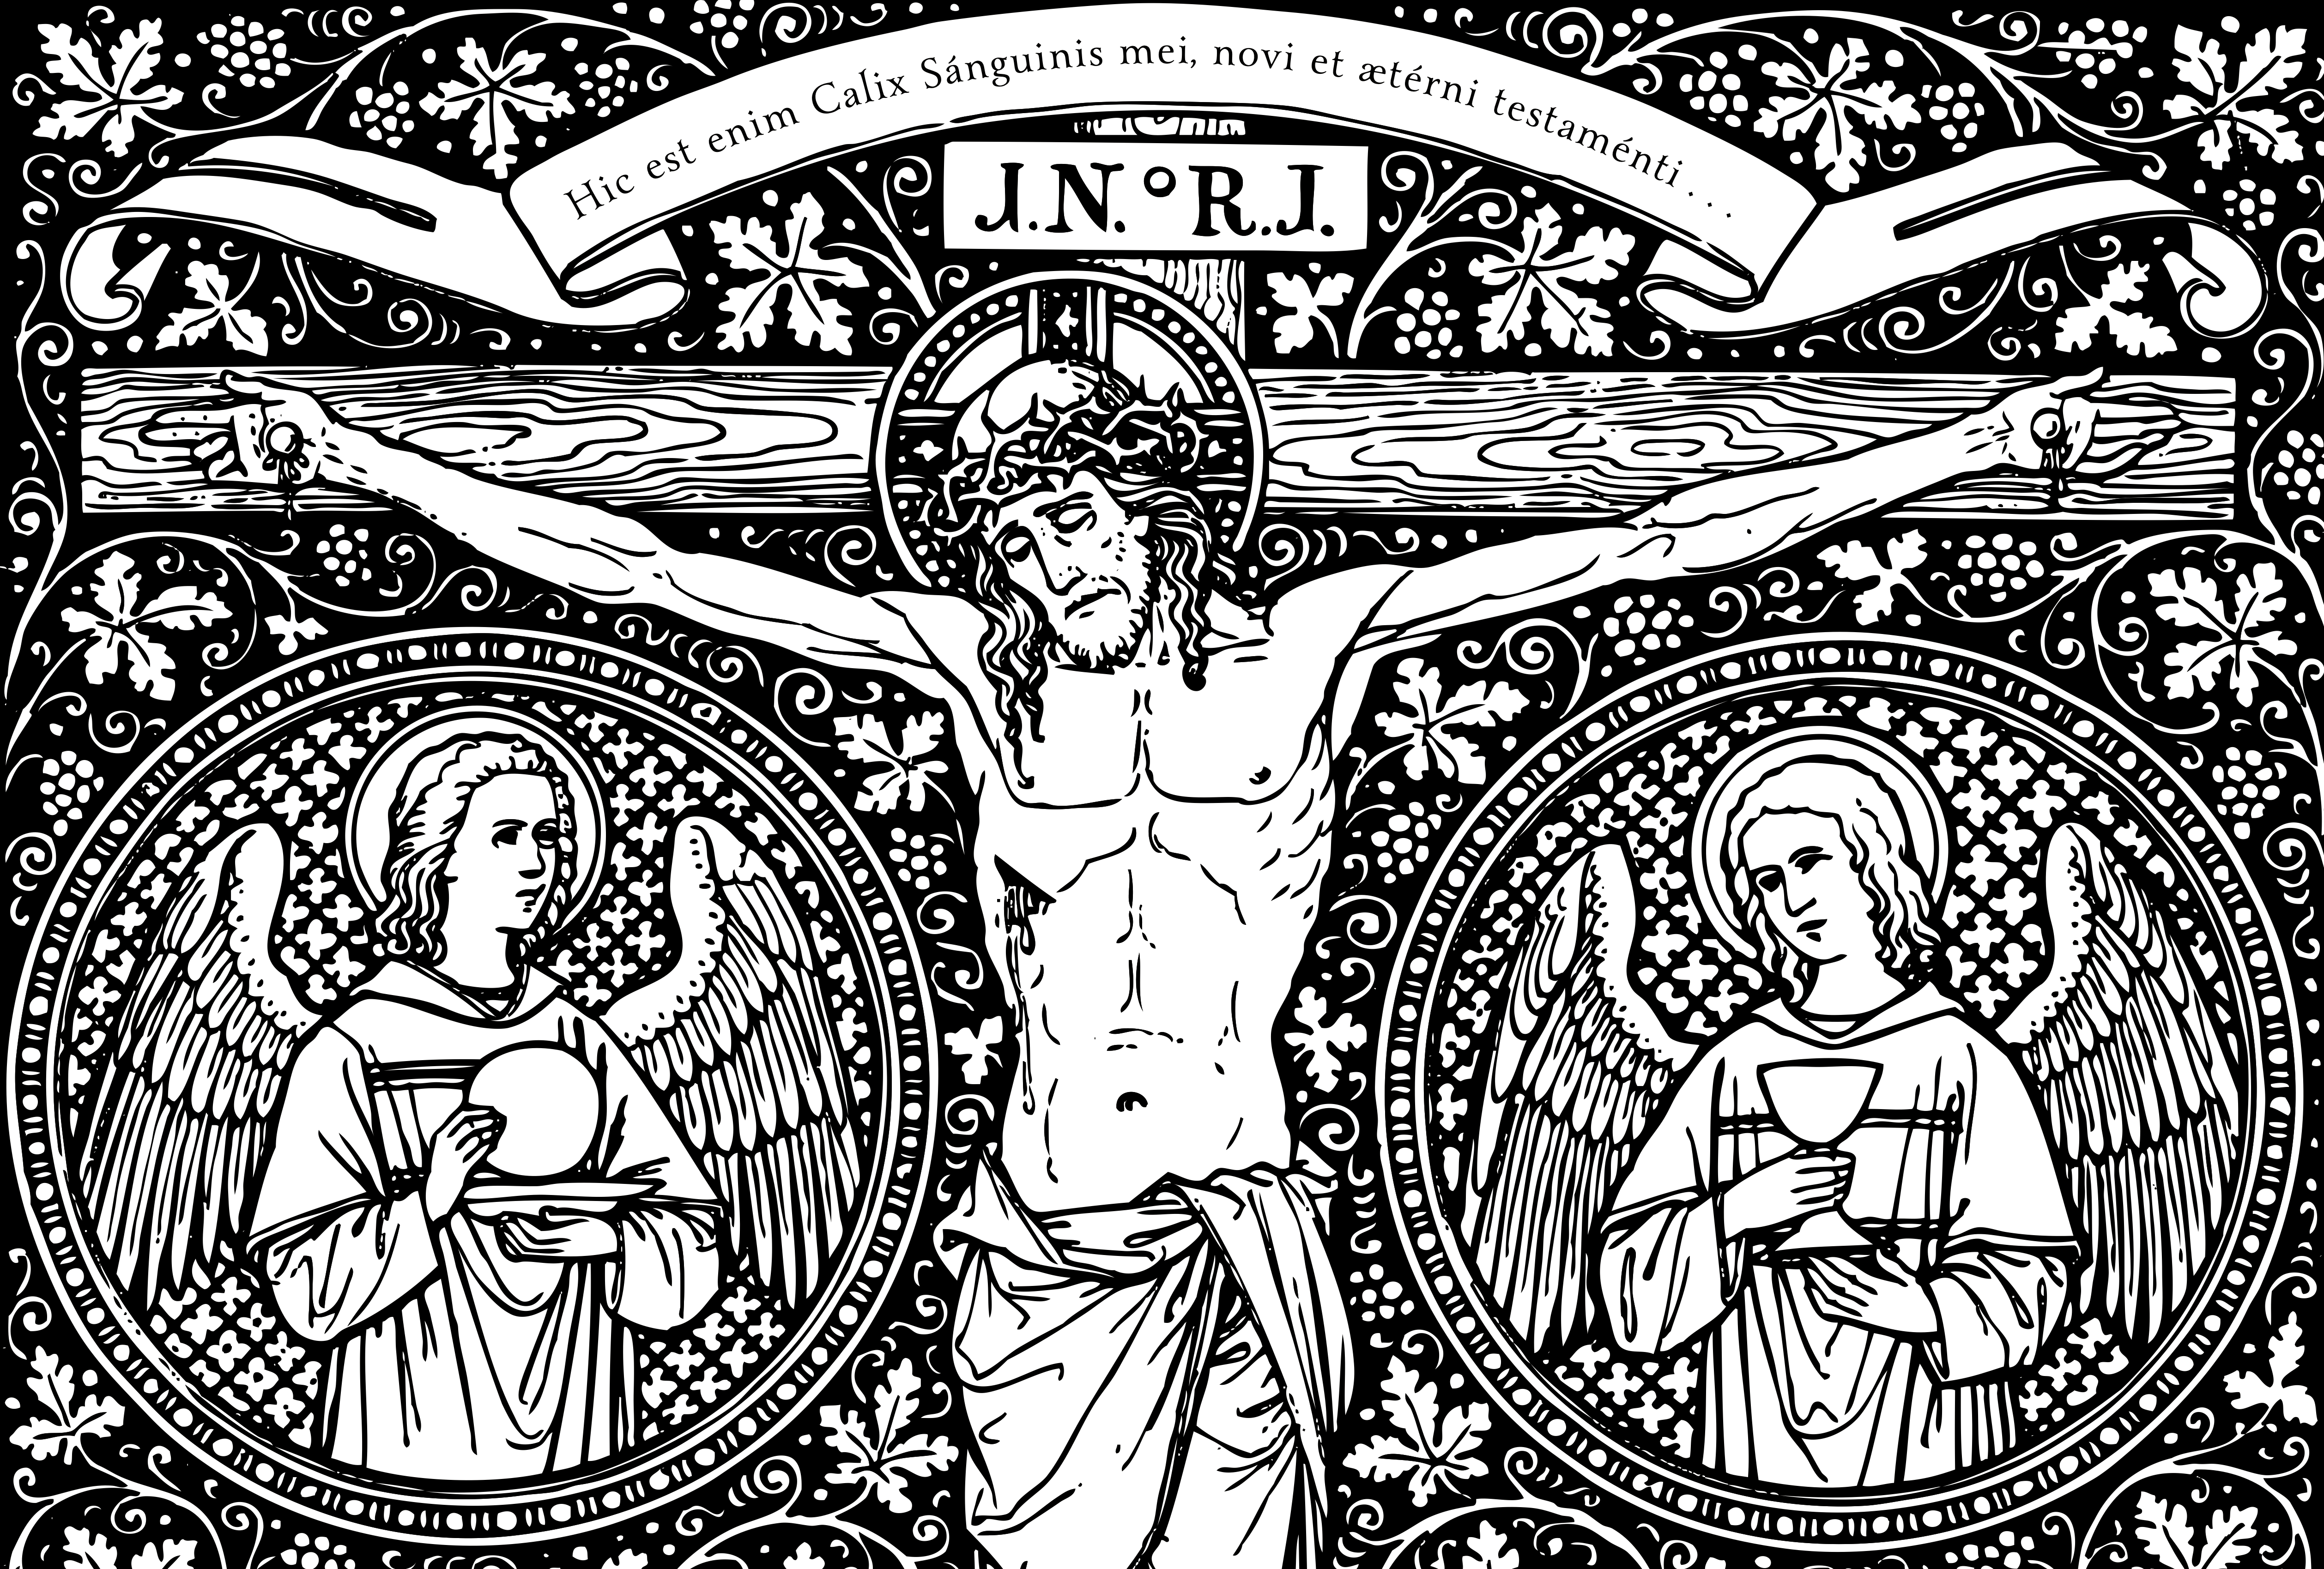
\includegraphics[width=\linewidth]{../Figures/krzyz.png}
		\end{center}
		%
		\bigskip
		%
		\lettrine[lines=3,depth=1]{\color{Maroon}Q}{\bfseries\color{Maroon}ui}
		pridie quam pateretur, accepit panem in~sanctas ac~venerabiles manus
		suas, et~elevatis oculis in~caelum ad~te Deum Patrem suum omnipotentem,
		tibi gratias agens, bene\cross dixit, fregit, deditque discipulis sui
		dicens: Accipite, et~manducate ex~hoc omnes:\\

		\medskip

		\centerline{\begin{minipage}{0.75\linewidth}
				\begin{center}
					\Large\color{Maroon}\bfseries\scshape
					%
					Hoc est enim Corpus meum.
				\end{center}
			\end{minipage}}

		\medskip

		\initial{S}{imili} modo postquam coenatum est, accipiens et~hunc
		praeclarum Calicem in~sanctas ac~venerabiles manus suas: item tibi
		gratias agens, bene\cross dixit, deditque discipulis suis, dicens:
		Accipite, et~bibite ex~eo omnes:\\

		\medskip

		\centerline{\begin{minipage}{0.75\linewidth}
				\begin{center}
					\Large\color{Maroon}\bfseries\scshape
					%
					Hic est enim Calix Sanguinis mei, novi et~aeterni
					testamenti: mysterium fidei: qui pro vobis et~pro multis
					effundetur in~remissionem peccatorum.
				\end{center}
			\end{minipage}}

		\medskip

		\centerline{\begin{minipage}{\linewidth}
				Haec quotiescumque feceritis, in~mei memoriam facietis.
			\end{minipage}}

	\end{minipage}
	\hspace*{0.8cm}
	\begin{minipage}[t]{0.29\linewidth}

		\vspace*{2.2cm}

		% \begin{minipage}{0.85\linewidth}
		% 	\initial{S}{uscipe}, sancte Pater, omnipotens aeterne Deus, hanc
		% 	immaculatam hostiam, quam ego indignus famulus tuus offero tibi Deo meo
		% 	vivo et~vero,
		% \end{minipage}
		% \vspace*{0.25em}

		\parbox{0.87\linewidth}{\initial{S}{uscipe}, sancte Pater, omnipotens
			aeterne Deus, hanc immaculatam hostiam, quam ego indignus famulus
			tuus offero tibi Deo meo vivo et~vero, pro}

		\smallskip

		innumerabilibus peccatis, et~offensionibus, et~negligentiis meis,
		et~pro omnibus circumstantibus, sed et~pro omnibus fidelibus Christianis
		vivis atque defunctis: ut~mihi, et~illis proficiat ad~salutem in~vitam
		aeternam.
		\amen

		\gap

		\initial{O}{fferimus} tibi, Domine, calicem salutaris, tuam deprecantes
		clementiam: ut~in~conspectu divinae majestatis tuae, pro nostra, et
		totius mundi salute cum odore suavitatis ascendat. \amen

		\gap

		\initial{I}{n} spiritu humilitatis, et~in~animo contrito suscipiamur a
		te, Domine: et~sic fiat sacrificium nostrum in~conspectu tuo hodie, ut
		placeat tibi, Domine Deus

		\gap

		\initial{V}{enite}, Sanctificator omnipotens aeterne Deus, et~bene\cross
		dic hoc sacrificium, tuo sancto nomini praeparatum.

		\gap

		\initial{S}{uscipe}, sancta Trinitas, hanc oblationem, quam tibi
		offerimus ob memoriam passionis, resurrectionis, et~ascensionis Jesu
		Christi Domini nostri: et~in~honorem beatae Mariae semper Virginis, et
		beati Joannis Baptistae, et~sanctorum Apostolorum Petri et~Pauli, et
		istorum, et~omnium Sanctorum: ut~illis proficiat ad~honorem, nobis autem
		ad~salutem: et~illi pro nobis intercedere dignentur in~caelis, quorum
		memoriam agimus in~terris. Per eumdem Christum Dominum nostrum. \amen

		\gap

		\initial{P}{laceat} tibi, sancta Trinitas, obsequium servitutis meae: et
		praesta; ut~sacrificium quod oculis tuae majestatis indignus obtuli,
		tibi sit acceptabile, mihique, et~omnibus, pro quibus illud obtuli, sit,
		te miserante, propitiabile. Per~Christum Dominum nostrum. \amen

	\end{minipage}
\end{center}

% \vspace*{1cm}

\end{document}
